%%%%%%%%%%%%%%%%%%%%%%%%%%%%%%%%%%%%%%%%%%%%%%%%%%
%%%%%%%%%%%%%%%%%%%%%%%%%%%%%%%%%%%%%%%%%%%%%%%%%%
%%
%% Based one the "beamer-greek-two" template provided 
%% by the Laboratory of Computational Mathematics, 
%% Mathematical Software and Digital Typography, 
%% Department of Mathematics, University of the Aegean
%% (http://myria.math.aegean.gr/labs/dt/)
%%
%% Adapted by John Liaperdos, October-November 2014
%% (ioannis.liaperdos@gmail.com)
%%
%% Last update: 22/06/2017 (English Support)
%% Source: https://es.overleaf.com/latex/templates/thesis-presentation-template-beamer-english-version-dpt-of-computer-engineering-technological-educational-institute-of-peloponnese/vwhtyshhtqmg
%%%%%%%%%%%%%%%%%%%%%%%%%%%%%%%%%%%%%%%%%%%%%%%%%%
%%%%%%%%%%%%%%%%%%%%%%%%%%%%%%%%%%%%%%%%%%%%%%%%%%
%%
\PassOptionsToPackage{unicode}{hyperref}
\PassOptionsToPackage{naturalnames}{hyperref}
\documentclass{beamer} 
\usepackage{babel}
\usepackage[utf8]{inputenc}
\usepackage{multicol}
\usepackage{caption}
\usepackage{subfig}


%%% FONT SELECTION %%%%%%%%%%%%%%%%%
%%% we choose a sans font %%%%%%%%%%
\usepackage{kmath,kerkis} 
%\usepackage[default]{gfsneohellenic} 
%%%%%%%%%%%%%%%%%%%%%%%%%%%%%%%%%%%%

\usepackage{color}
\usepackage{amsmath}
\usepackage{amssymb}

\usepackage{epstopdf}
\usepackage{graphicx}
\graphicspath{{./img/}}

%%
% load TEI-Pel - specific layout
\usepackage{TeiPel_En_Beamer_Layout}
\setTeipelLayout{draft,newlogo}% options: "draft", "newlogo"

%%%%%%%%%%%%%%%%%%%%%%%%%%%%%%%%%%%%%%%%%%%%%%%%%%%%%%%%%%%%
% Thesis Info %%%%%%%%%%%%%%%%%%%%%%%%%%%%%%%%%%%%%%%%%%%%%%
%%%%%%%%%%%%%%%%%%%%%%%%%%%%%%%%%%%%%%%%%%%%%%%%%%%%%%%%%%%%
	% title
		\title[Análisis de redes causales en deportes de equipo]{Análisis de redes causales en deportes de equipo}	
	% author 
    % (In the mandatory argument "{}", separate multiple
    % authors with "\and" - use "\\" for better author name formatting
    % in the title page. In the optional argument "[]" include all
	% author names, with no "\and" or text formatting macros.)
	% Example: 
    %\author[A. Author Albert Einstein]{Anthony Author \and Albert Einstein}
		\author[E. Merelo]{Elena Merelo}
	% supervisor	
		% \supervisor{Supervisor}{Mister Supervisor}{Professor}
	% date
		\presentationDate{7 de septiembre de 2022}
%%%%%%%%%%%%%%%%

\begin{document}

% typeset front slides
	\typesetFrontSlides

%%%%%%%%%%%%%%%%
% Your Slides Start here:

%%%%
\section{Introducción}

%%
\subsection[Problema]{Descripción del problema}

\begin{frame}{Motivación}
	\framesubtitle{El fútbol es un deporte de equipo \textit{complejo}}
    Como parte del cuerpo técnico de un equipo habrá que decidir:
    \begin{itemize}
		\item Quiénes jugarán
		\pause
		\item Dónde se posicionarán
		\pause
        \item Cuándo y qué cambios habrá
		\pause
        \item Alineación por la que se abogará
        \pause
        \item A quién fichar o vender, qué hacer en los entrenamientos,... 
	\end{itemize}
\end{frame}

\begin{frame}{Descripción}
	\begin{itemize}
		\item <1->¿Analizar la entropía sobre el grafo de pases nos ayuda a entender mejor el desempeño de un equipo?
		\item <2->¿Hasta qué punto es determinante la entropía a nivel de jugador o equipo?
        \item <3->¿Es posible ver la entropía reflejada en un tipo de visualización de las redes de pases?
	\end{itemize}
\end{frame}

\begin{frame}{Metodología}
	\begin{itemize}
		\item \textbf{Desarrollo ágil}
		\pause
		\item \textit{Design thinking}
	\end{itemize}
\end{frame}

%%
\subsection{Definiciones}
\begin{frame}{Grafos}
	\begin{definition}
		Un grafo es un par $\mathcal{G} = (V, E)$, con $V$ conjunto finito de vértices distinguibles y 
		$E \subseteq V \times V$ conjunto de aristas. Un par ordenado $(u, v) \in E$ denota un borde dirigido
		del vértice $u$ al vértice $v$, y se dice que $u$ es padre de $v$ y $v$ hijo de $u$. Los bordes dirigidos 
		se representarán con flechas. 
	\end{definition}
\end{frame}

\begin{frame}{Redes bayesianas}
	\begin{center}
		Ejemplo de grafo dirigido acíclico \\[12pt]
		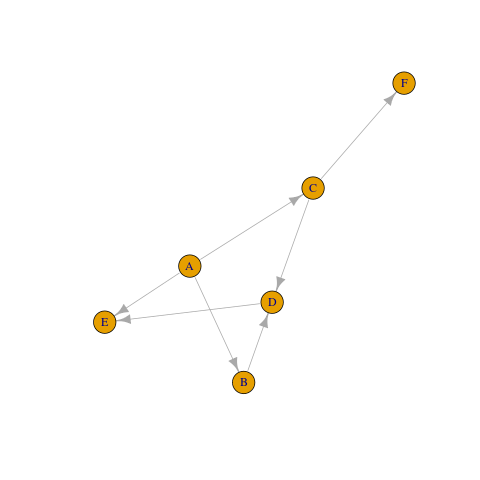
\includegraphics[width=0.35\textwidth,keepaspectratio]{dag.png}
		\\
		\footnotesize(Una red bayesiana consiste en un modelo estructural y un conjunto de probabilidades)
    \end{center}
\end{frame}

\begin{frame}{Entropía}
	\begin{definition}[Entropía] \label{def:entropy}
        Para $X$ variable aleatoria discreta:  
        
        $$H(X):= - \sum_{x} P(x)\log[P(x)]$$
        
        donde $X$ toma valores en $\mathcal{X}$, $P:\mathcal{X} \rightarrow [0,1]$.
        La entropía conjunta de las variables $X_1...X_N$ se define por 
        $$H(X_1,...,X_N):=-\sum_{x_1}...\sum_{x_N}P(x_1,...,x_N)\log[P(x_1,...,x_N)]$$
    \end{definition}
	\begin{example}
	Nosotros calificaremos a los equipos según la entropía obtenida de las redes de pases entre los jugadores, 
 	la cual caracteriza su grado de uniformidad o variabilidad.
	\end{example}
\end{frame}

%%%%
\section{Contribuciones}

%%
\subsection{Resultados}

\begin{frame}{Redes de pases a lo largo de la competición}
    \begin{columns}[t]
        \column{.5\textwidth}
        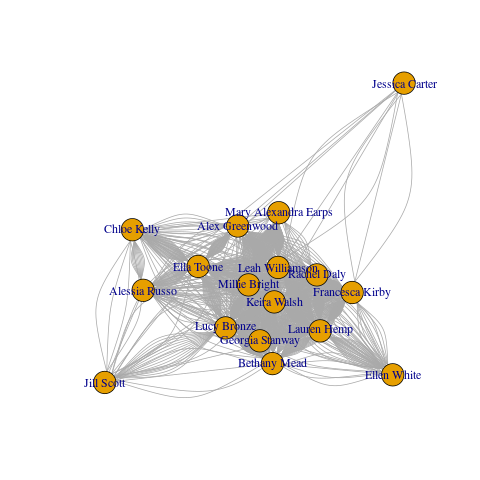
\includegraphics[width=\columnwidth,height=3cm]{plot_england.png}
        \captionof{figure}{Red de pases total de Inglaterra}
        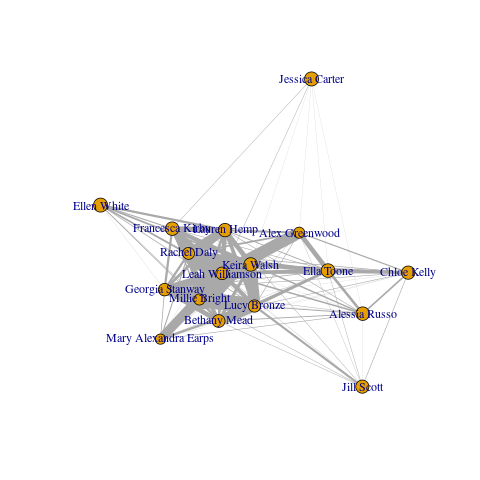
\includegraphics[width=\columnwidth,height=3cm]{plot_england_simpl.png}
        \captionof{figure}{Red de pases total simplificada de Inglaterra}
        \column{.5\textwidth}
        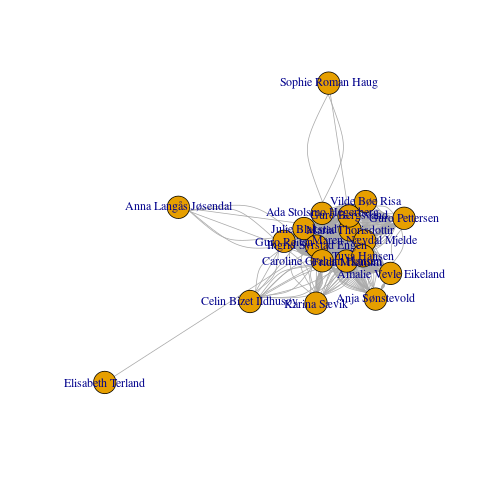
\includegraphics[width=\columnwidth,height=3cm]{plot_norw.png}
        \captionof{figure}{Red de pases total de Noruega}
        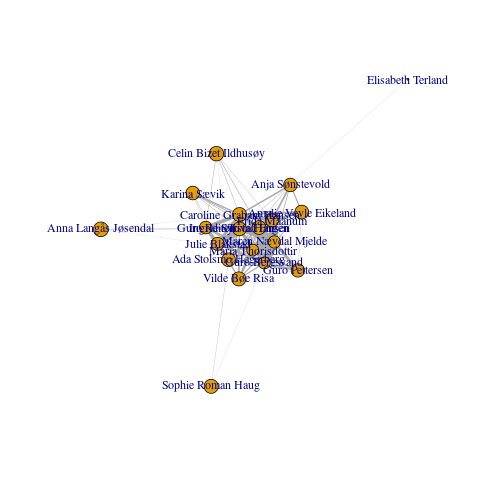
\includegraphics[width=\columnwidth,height=3cm]{plot_norw_simpl.png}
        \captionof{figure}{Red de pases total simplificada de Noruega}
    \end{columns} 
	\begin{alertblock}{Nota}
		\textlatin{En las simplificaciones, la entropía por jugadora es el tamaño de cada nodo. El grosor de los enlaces es el 
	 	número de pases que ha habido.}
	\end{alertblock}
\end{frame}

\begin{frame}{Partido Inglaterra - Noruega}
		\begin{columns}[t]
			\column{.5\textwidth}
			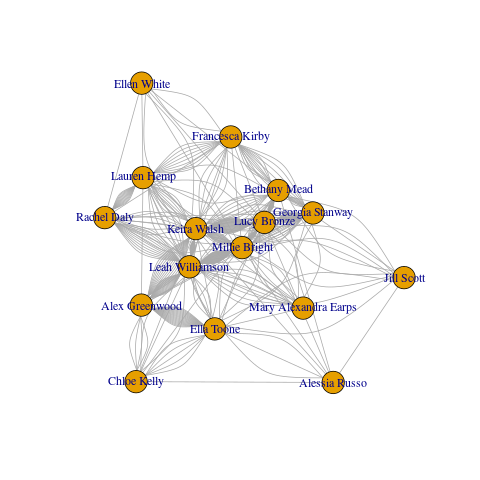
\includegraphics[width=\columnwidth,height=3cm]{entropy_match_eng.png}
			\captionof{figure}{Entropía conjunta de Inglaterra}
			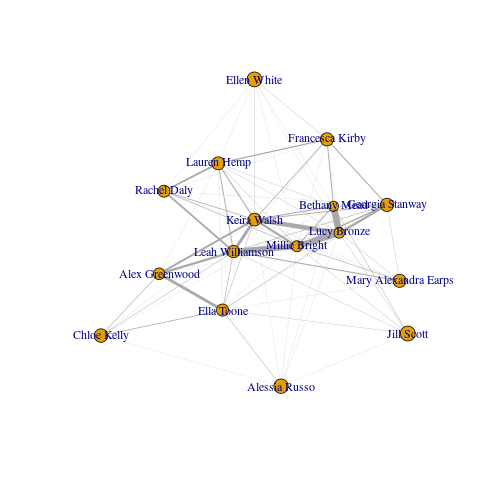
\includegraphics[width=\columnwidth,height=3cm]{entropy_match_engl_simpl.png}
			\captionof{figure}{Entropía conjunta simplificada de Inglaterra}
			\column{.5\textwidth}
			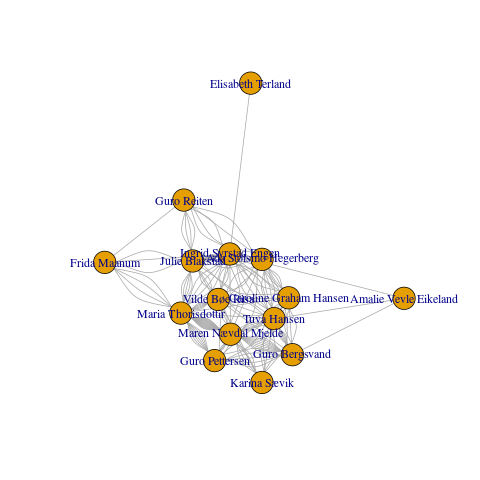
\includegraphics[width=\columnwidth,height=3cm]{entropy_match_norw.png}
			\captionof{figure}{Entropía conjunta de Noruega}
			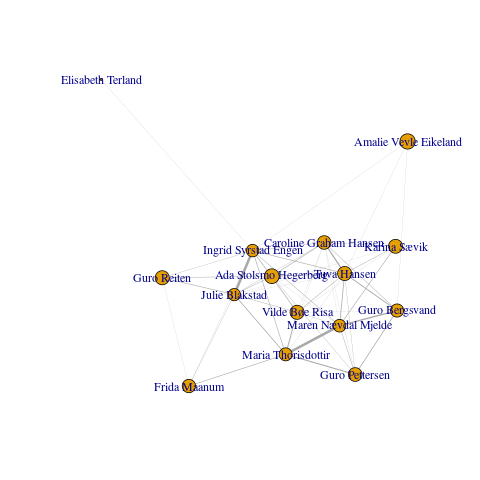
\includegraphics[width=\columnwidth,height=3cm]{entropy_match_norw_simpl.png}
			\captionof{figure}{Entropía conjunta simplificada de Noruega}
		\end{columns} 
	\end{frame}

\begin{frame}{Comparativa por jugadoras}
	\begin{figure}
		\centering
		 \subfloat[Entropía total Inglaterra]{
		   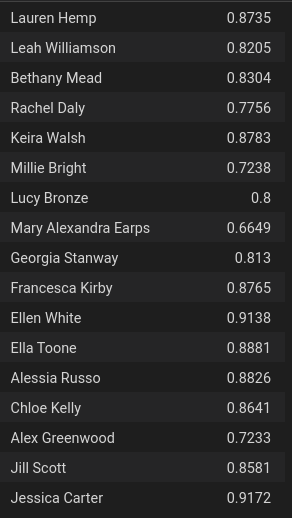
\includegraphics[width=0.2\textwidth]{table_entrop_engl.png}}
		 \subfloat[Entropía en el partido Inglaterra]{
		   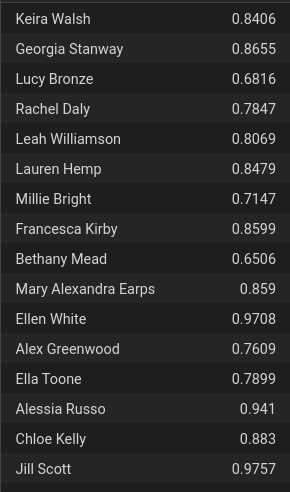
\includegraphics[width=0.2\textwidth]{table_entropy_match_eng.png}}
		 \subfloat[Entropía total Noruega]{
		   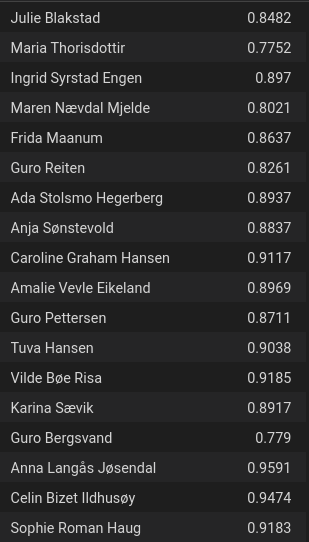
\includegraphics[width=0.2\textwidth]{table_entrop_norw.png}}
		\subfloat[Entropía total en el partido Noruega]{
			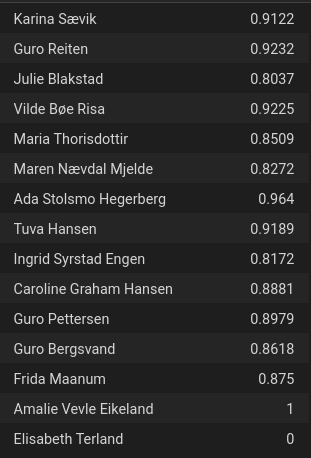
\includegraphics[width=0.2\textwidth]{table_entropy_match_norw.png}}
	   \end{figure}
\end{frame}

%
\subsection{Conclusiones y trabajos futuros}

\begin{frame}{Conclusiones}
	\begin{itemize}
		\item Equilibrio entre organización y desorganización
		\item Menos entropía, más comunicación
		\item Más entropía, más grados de libertad 
		\item Una entropía lineal alta muestra un peor desempeño
	\end{itemize}
\end{frame}

\begin{frame}{Trabajos futuros}
	Introducción de redes bayesianas para:
	\begin{itemize}
		\item Adaptación al rival
		\item Posesión del balón
		\item Minutos jugados
		\item Entropía espacio-temporal
		\item Alineación y cambios
	\end{itemize}
\end{frame}

\subsection{Extra}

\begin{frame}{Costes}
	\begin{table}
		\begin{tabular}[h!tbp]{lccr}
		  Concepto & Coste unitario & Unidades & Total \\
		  Amortización portátil & 150€ & 1 & 150€ \\
		  Ventilador            & 12€  & 1 & 14€ \\
		  Costes laborales      & 2000€& 3.5 & 7000€ \\
		  \hline \\
		  \multicolumn{3}{l}{Total} & 7164€ \\
		\end{tabular}
		\caption{Costes el proyecto en el escenario ``analista de datos junior''} \label{tab:costes2}
	\end{table}
\end{frame}

\begin{frame}{Asignaturas usadas}
	\begin{itemize}
		\item Estadística descriptiva e introducción a la probabilidad 
		\item Inferencia estadística 
		\item Probabilidad 
		\item Estadística computacional 
		\item Infraestructura Virtual
	\end{itemize}
\end{frame}

\begin{frame}{Sobre los datos usados}
	\begin{itemize}
		\item \href{https://statsbomb.com/articles/soccer/statsbomb-release-free-360-data-womens-euro-2022-available-now/}{StatsBomb 360}
		captura la posición de todos los jugadores por cada evento que ocurre.
	\end{itemize}
	\begin{center}
		Fuente de los datos \\[12pt]
		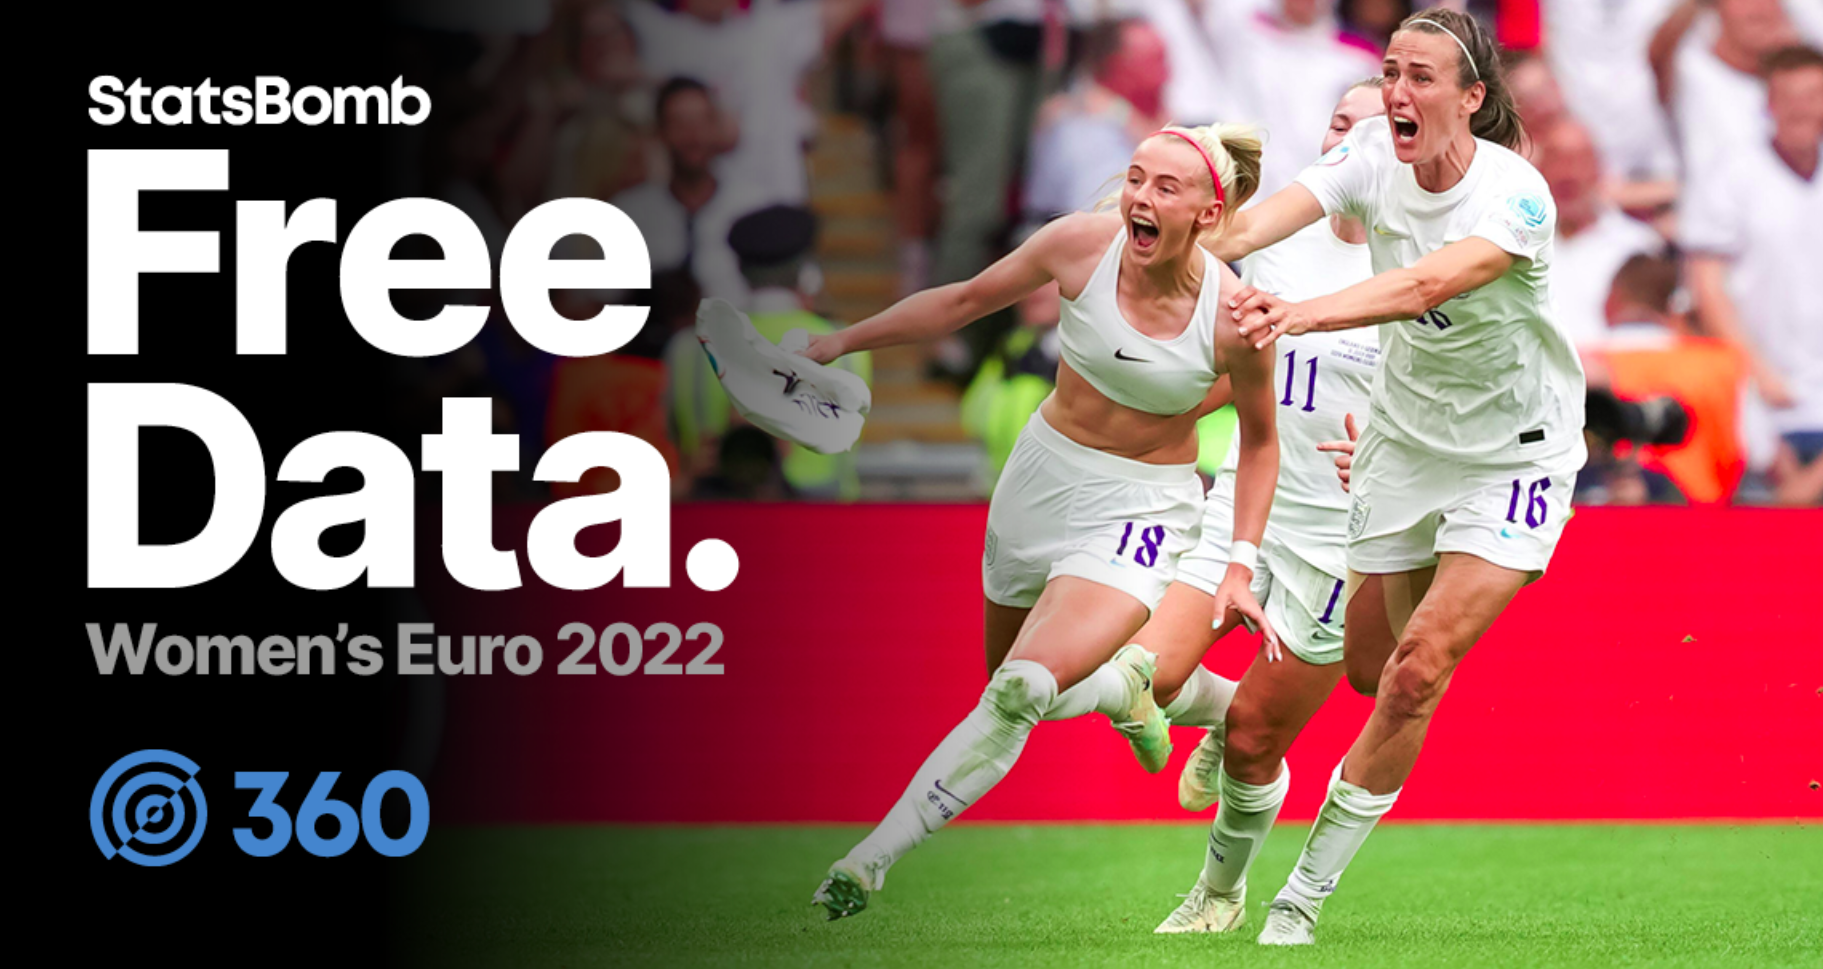
\includegraphics[width=0.35\textwidth,keepaspectratio]{free_data.png}
		\\
		\footnotesize(Nunca antes se había liberado datos 360 de StatsBomb para fútbol femenino)
    \end{center}
\end{frame}

\begin{frame}{Redes bayesianas}
    \begin{definition}[Redes bayesianas] 
        Una red bayesiana $\mathfrak{B} = \lbrace \mathcal{G}, \mathbb{P} \rbrace$ está definida por:
        \begin{itemize}
            \item $\mathcal{G}=(V,E)$ 
            \item $(\Omega, \mathbb{P})$.
            \item $\textbf{V}=V[i], i=1,...,N$, $(\Omega, \mathbb{P})$ 
            de tal manera que $\mathbb{P}(V[1],...,V[N])= \prod_{i=1}^{n}\mathbb{P}(V[i]|pa(V[i]))$
        \end{itemize}
    \end{definition}     
\end{frame}

\begin{frame}{Redes causales}
   \begin{block}
        <1->{}
            \begin{itemize}
                \item Red bayesiana en la que los padres de cada nodo son sus causas directas.
                \item Satisface la {\em condición de Markov causal}
            \end{itemize}
    \end{block}
    \begin{exampleblock}
        <2->{Condición de Markov causal}
            \begin{itemize}
                \item Dadas las causas directas, el fenómeno asociado a un nodo es independiente de 
                los que no tienen efecto sobre él. Esta asunción permite que la distribución 
                conjunta de las variables en una red causal sea factorizada como :
                $$ P(X_{1}, \dots,X_{N}) = \prod_{i=1}^{N} P(X_{i} | pa(X_{i}))$$ 
            \end{itemize}
    \end{exampleblock}
\end{frame}

\begin{frame}{Bibliografía}
	\begin{thebibliography}{2}
		\beamertemplatebookbibitems
		\bibitem{pgm}C.\ Rohilla. \newblock\emph{Advanced Data Analysis from an elementary point of view}.\newblock
\textlatin{Some Press, \oldstylenums{1990}}.

		\beamertemplatearticlebibitems
		\bibitem{Someone2002}B.\ Author.\newblock On this and that\emph{.}
\newblock\emph{Journal on This and That}. 
\oldstylenums{2}(\oldstylenums{1}):\oldstylenums{50}--\oldstylenums{100}, 
\oldstylenums{2000}.
	\end{thebibliography}
\end{frame}

%%
\end{document}